%% ----------------------------------------------------------------
%% Overlay.tex
%% ----------------------------------------------------------------

\chapter{Overlay - vgQuestions} \label{Chapter:Overlay}

\begin{preamble}
A videogular plugin was written to provide the core functionality. It allows for questions to be overlaid on top of the video and handles user interaction.

This plugin is called videogular-questions or \gls{vgQuestions} for short.

It provides a utility library which wraps the messaging passing interface making it easy to create content (used for the \gls{DF}).

\end{preamble}

\section{Introduction}

This plugin was one of the primary focusses of the project, an accessible system presenting the user with questions overlaid on a video. A number of features were explicitly requested by the client such as question types (\cref{Req:Question types}) and the ability to let users re-watch content easily if questions were answered incorrectly (\cref{Req:Jumping to content}).

\section{Design}

\begin{figure}[h]
\makebox[\textwidth][c]{
\begin{tikzpicture}[
  font=\sffamily,
  every matrix/.style={ampersand replacement=\&,column sep=1.6cm,row sep=1.6cm},
  source/.style={draw,thick,rounded corners,fill=yellow!20,inner sep=.3cm},
  vg-plugin/.style={draw,thick,rounded corners,fill=yellow!20,inner sep=.3cm},
  analytics-frontend/.style={draw,thick,rounded corners,fill=red!20,inner sep=.3cm},
  videogular/.style={draw,thick,circle,fill=blue!20},
  process/.style={draw,thick,circle,fill=blue!20},
  sink/.style={source,fill=green!20},
  datastore/.style={draw,very thick,shape=datastore,inner sep=.3cm},
  server/.style={source,fill=green!20},
  dots/.style={gray,scale=2},
  to/.style={->,>=stealth',shorten >=1pt,shorten <=1pt, semithick,font=\sffamily\footnotesize},
  between/.style={<->,>=stealth',shorten >=1pt,shorten <=1pt,semithick,font=\sffamily\footnotesize},
  every node/.style={align=center}]

  \matrix{
    \node[videogular] (videogular) {videogular}; \&
    \node[vg-plugin] (vg-questions) {vgQuestions}; \&
    \node[vg-plugin] (questions-worker) {questions-worker.js}; \&
    \node[server] (quiz) {quiz.js}; \\
  };

  \draw[to] (videogular.-20) --
      node[midway,below] {video states} (vg-questions.195);
  \draw[to] (vg-questions.-195) --
      node[midway,above] {command} (videogular.20);

  \draw[to] (vg-questions.-14) --
      node[midway,below] {user interactions} (questions-worker.190);
    \draw[to] (questions-worker.-190) --
      node[midway,above] {commands} (vg-questions.14);

  \draw[to] (questions-worker.-10) --
      node[midway,below] {utility function} (quiz.201); 
  \draw[to] (quiz.-201) --
      node[midway,above] {quiz description} (questions-worker.10);
\end{tikzpicture}
}
\caption{vgQuestions Architecture}
\label{Figure:vgquestions-architecture}

\end{figure}

The core of \gls{vgQuestions} is a \gls{DF} that is loaded in a \gls{webworker} that will talk to \gls{vgQuestions} as shown in \autoref{Figure:vgquestions-architecture}. This uses a well defined message passing interface to allow easy communication. As the \gls{DF} is provided by the user this makes the plugin exceptionally flexible. Many items of this can easily be changed to create a dynamic set of questions however most users will not interact with this directly.

The general use case is that the \gls{DF} will be generated through use of the authoring tool however the ability to manually create this file is open. This lets the user interface with the questions-worker.js library and configure the actions of the questions. The questions-worker.js library handles communication with vgQuestions, loading a JavaScript object that contains description of the quiz.

\section{Implementation}
The implementation of the overlaid video player was split into three sections. The first was deciding how to represent the question sets internally. Next was how to represent the questions within the user interface. The final section was implementing the back end communication between the question representations and the video.

\subsection{Annotations}
\label{Section:Annotations}

One of the main issues to address early on was how to represent the quiz and poll questions. The \gls{QTI} specification was investigated, but was found to be complicated and incomplete \todo{What does incomplete mean here?} for the project needs. It was decided to design a new format for representing the data and logic that is used for a particular application of videogular-questions.

This new format separates the front end of the library (responsible for interacting with the \gls{DOM}), from the data and logic regarding the questions by means of a message passing interface. This is achieved in a rigorous way in the browser by means of a \gls{webworker}. This is a sandboxed separate thread that runs in the background of the webpage. They run independently of standard user-space scripts.  More can be found out about their use within this project in \autoref{Subsection:WebWorkers}

Using JavaScript, rather than a pure data representation (e.g. JSON or XML) allows you to include logic for the application to follow. This makes it extremely flexible and concise, and the isolation provided by the \gls{webworker} mitigates many security concerns with having an application that executes data given as input as code.

Every item in an annotation can have an action and condition function. The action function is called when a item finishes. The action function is given the state of the annotations, such that it can make decisions and then affect the state of the video accordingly. For example, in the above example, this is used to only have the ``skip back" question show, if the answer given to the previous question is incorrect.

The condition function is called to determine if the respective item will show. By default, when an annotation is shown, each item is shown in sequence. However, if an item has a condition function, this is evaluated, and the item only shown if the condition function returns \lstinline|true|. If the condition function returns \lstinline|false|, the item is skipped. This functionality is used in the above example to have the video skip back if the user wants it to.

An early decision was to define the difference between a poll and a quiz question. The decision made was that a poll is a type of quiz question that does not have a correct answer.

Initially basic question types (single choice, multiple choice and scale questions) were focused on. A variety of visualisations was implemented including check boxes, radio buttons and sliding scales. Validation was needed to ensure that the specified minimum and maximum limits were followed.

By having a standard \gls{DF} that uses JavaScript functions it was possible to write template functions that could be outputted from the authoring tool and read by the overlay correctly.

In reviewing the types of questions we would support we produced a class diagram (\autoref{Figure:questions_class_diagram}) to represent the type of data that the questions would have. Once the additional question types of textual and range were implemented this gave us conformance to \cref{Req:Question types}.

If the \lstinline|record_response| type was set to a \lstinline|true| value, the question would become a poll and report back the results to a server. If the \lstinline|correct_answer| attribute was set then the question would have a true value and would be shown to the user, if requested. This allows a user to possible have a poll type question that stores the data collected and also has a right answer. This provides maximum usability and therefore doesn't distinguish between a quiz or a poll in the underlying code.

Single question is a sub type of Multiple question where min and max (the minimum and maximum selected number of answers) is 1.

Similarly, the stars question is similar to the range question where the \lstinline|step value| is 1.

\autoref{code:questionworker} shows an example of the quiz definition file that could be used by the Videogular Questions plugin.

\begin{figure}
\centering
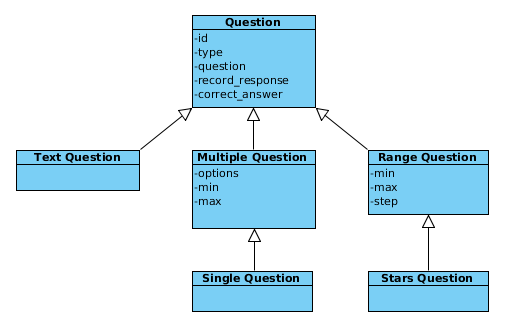
\includegraphics[width=12cm]{../figures/questions_class_diagram.png}
\caption{A class diagram representing what attributes each question type needs to detail}
\label{Figure:questions_class_diagram}
\end{figure}

\subsection{Front End - User Interface}

The appearance of the overlay depends on the question type to be shown. The layout of these different types was carefully considered for accessibility and ease of use. Mockups were made and user studies were done in collaboration with a third year project student.

A set of example \gls{CSS} files are supplied with the project that layout the questions according to the feedback received. Developers using any part of the project can use these styles as is, or modify/develop their own.

\subsection{Back End - WebWorkers}
\label{Subsection:WebWorkers}

\Glspl{webworker} give a good way of running (sandboxed) background scripts that are computationally intensive. They are a way of multithreading - allowing multiple scripts to run simultaneously, avoiding the problem of unresponsive pages due to long running scripts. This is done by using message passing.

For example, when an answer is submitted by the user this would sent a message to the \gls{webworker} containing the answer. The \gls{webworker} can then process this information without affecting the responsiveness of the page. Once the processing is complete the \gls{webworker} can send a message back to the page to tell it what to do next.

\begin{figure}

\centering

\begin{sequencediagram}
  \newthread[white]{c}{Front End}
  \newinst[4]{s}{WebWorker}

  \mess{s}{annotations}{c}

  \stepcounter{seqlevel}
  \begin{call}
    {c}{annotationStart}
    {s}{showQuestion}
  \end{call}

  \stepcounter{seqlevel}
  \begin{call}
    {c}{questionResult}
    {s}{showQuestion}
  \end{call}

  \stepcounter{seqlevel}
  \begin{call}
    {c}{questionResult}
    {s}{endAnnotation}
  \end{call}
\end{sequencediagram}
\caption{Sequence diagram showing interactions between the front end and webworker}
\label{Figure:sequence_diagram_frontend_webworker}

\end{figure}

\autoref{Figure:sequence_diagram_frontend_webworker} illustrates messages that could pass between the \gls{webworker}, and the front end when the above example is used. Initially, the worker sends an \lstinline|annotationStart| message which contains the times which annotations will occur.

When the first time is reached, the front end sends a \lstinline|annotationStart| message to the worker, containing the id of that annotation. The worker then replies with a \lstinline|showQuestion| message, containing the contents of the first question. Note that here, the functions are not sent to the front end, just the JSON representation of the question is sent.

When the user responds to the question, that response is send to the worker in a \lstinline|questionResult| message. In this case, the user responded incorrectly, therefore, when the \gls{webworker} evaluated the condition on the second question, it evaluated to \lstinline|false|. This meant that the worker replied with another \lstinline|showQuestion| message.

Once the user responds to the second question, the response is again sent to the \gls{webworker}. In this case, this was the final question in the annotation, so the worker responds with an \lstinline|endAnnotation| message.

\section{Conclusion}
An internal representation of the questions is given by the \acrlong{DF} that is used to display the questions to the user in the overlays. \gls{CSS} is used to keep the appearance of the questions consistent. \Glspl{webworker} are used to communicate with the front end to provide the necessary messages for the expected actions to occur.